\documentclass[]{article}

%opening
\usepackage[pdftex]{graphicx}
\usepackage[options ]{algorithm2e}
\title{Draft Review State of The Art }
\author{}

\begin{document}

\maketitle

\begin{abstract}

\end{abstract}

\section{Introduction Draft}

The infiltration of Internet into day to day applications led to the explosion of data within different acitivty sectors. Therefore the need to group these data and extract pertinant information became necessary. Recent studies have shown that the big four (Google, Amazon, Microsoft and Facebook) alone hold more than 1200 petabytes of data, 1 petabyte is equal to 1000 terabytes and each terbayte to 1000 gegabytes, excluding other big data holders as DropBox...

\noindent The increase in both volumr and variety of data requires advances in methodology to automatically understand, process and summarize the data\cite{jain2008data}.This growth of the amount of information being circulated between users all over the globe made the need for grouping this information really urgent. This kind of grouping is called data analysis which can be concerned with predictive modeling: Being given some training data we want to predict the behavior of the unseen test data. This task is defined as learning, often there is a clear distinction between learning problems that are defined into two categories 

\begin{itemize}
 \item Supervised learning also known as classification, in the context of artificial intelligence (AI) and machine learning, is a type of system in which both input and desired output data are provided. Input and output data are labelled for classification to provide a learning basis for future data processing.
 \item Unsupervised learning also known as clustering, which is a type of machine learning algorithm used to draw inferences from datasets consisting of input data without labeled responses. 
\end{itemize}

\noindent In other words, the difference between the methods presented before is that for classification the class labels are known by the user. On the other hand clustering is more challenging than classification for the simple reason that the class labels ar not predefined and they will be known over time. Semi-supervised learning which is a hybrid model\cite{chapelle2006continuation} consisting on a combination of classification and clustering: only a small set of the training data is labeled.

Every second, approximately 6,000 tweets are tweeted; more than 40,000 Google queries are searched; and more than 2 million emails are sent, according to Internet Live Stats, a website of the international Real Time Statistics Project. This information leads us to the conclusion that Big Data is in constant for mining and therefore clustering and classification.
\noindent The challenge in the process of learning Big Data lies on the fact that most of the applications are online therefore the stream of data is represented by a contious flow. This led to both classification and clustering algorithms that function in an online and incremental way in order to be able to handle continuous data streams.

The aim of these learning techniques is to extract potentially useful knowledge from data streams which is a big challenge since most of the data mining techniques suppose that there is a finite amount of data that can be physically stored and analyzed. For data stream mining, however, the successful development of online incremental clustering and/or classification methodologies has to take into account the foollowing restrictions\cite{silva2013data}:
\begin{itemize}
	\item Data objects arrive contiously;
	\item There  is no specific order of arrival of the data;
	\item The size of the data stream cannot be predefined;
	\item Important data can be discarded over time;
	\item The distribution may change over time;
\end{itemize}

The rest of this paper will be organised in the follow way: in section 2 we will include the extended definition of clustering, a historical overview of the clustering algorithms and there development till today, and presentation of the latest incremental online clustering technologies. Section 3 will include an extended definition of data classsification, a historic overview of classification methods and the lastest online incremental classification methods along with there necessity.

\section{Static Data Analysis}

 The rest of the paper will be organised as follows: Detailed presentation of static data, extended definition of both clustering and classification of data.

\subsection{Static Data Definition}
Data can be divided into two major types: Static data which can be defined by the fact that these data occupy a limited space memory wise and this type of data doesn't vary with time. On the other hand there is dynamic data streams which will be presented in detail throughout this paper.
\subsection{Clustering definition}
Clustering can be considered the most important unsupervised learning problem; so, as every other problem of this kind, it deals with finding a structure in a collection of unlabeled data. A loose definition of clustering could be “the process of organizing objects into groups whose members are similar in some way”. A cluster is therefore a collection of objects which are “similar” between them and are “dissimilar” to the objects belonging to other clusters.

An alternative definition of clustering can be defined by the following: givern a representation of n objects, find K groups based on a measure of similarity such that the measure of similarity between the data that belong to a same cluster presents a high score while the same parameter should show a low value when the case is represented by data in different groups.

In the current digital era, according to (as far) massive progress and development of the internet and online world technologies such as big and powerful data servers, we face a huge volume of information and data day by day from many different resources and services which were not available to humankind just a few decades ago. Services over the world wide web are providing big masses of data: such as Facebook, Twitter, Youtube... that should be handled, therefore the need of clustering algorithms that can group these data and help make an extraction of useful information.\cite{fahad2014survey}

A search via google Scholar\cite{gsc} for the sequence data clustering has gotten 3,1 million scientific documents attached to this domain. This vaste litterature shows the importance of data clustering and taking into consideration from 2013 509 thousands results which corresponds to 16 percent of the total documents.

\begin{figure}[h!]
	\centering
	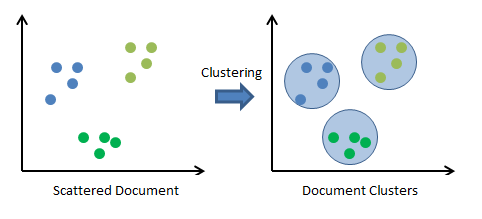
\includegraphics[width=0.5\textwidth]{clustering.png}
	\caption{Clustering: The process of regrouping showing high similarities into separate coherent groups}
\end{figure} 

From basic infromation retrieval applications to resolving cases in forensics data clustering can be considered vital for many reasons:

\begin{itemize}
	\item Permits the extraction of the underlying structure of the data being processed: gaining insight into the data, generating hypotheses, detecting anomalies...
	\item Another reason relies in determining the level of similarity among the studied data.
	\item Summarizing the data therefore being able to compress it in order to get the general idea with a considerable reduction within space and time.
\end{itemize}
\subsubsection{From then till now}
The term clustering first was used in 1954 in the anthropological domain. Several nominations existed throughout the time for the term clustering depending on the domain in which it was used\cite{jain1988algorithms}. Multiple books have treated the subject of clustering in detail and were cited enormously by researchers for their authenticity and contributions. Those books gave a deeper image of what clustering is and how it can be used in the aspects of daily life as well as in research:Hartigan \cite{hartigan1975clustering} defined in detail what clustering is in his book and discussed multiple application domains for its application. Since then the link between clustering and data mining was made and became a subject of research and study and was best elaborated in Han and Kamber 2000 \cite{han2000data}. Next to data mining machine learning, which can be presented as a type of artificial intelligence (AI) that provides computers with the ability to learn without being explicitly programmed. Machine learning focuses on the development of computer programs that can change when exposed to new data, also used the presence of data clustering in order to help develop artificial intelligence algorithms aiming to achieve the automation and independance of computers especially in pattern recognition which is well described in \cite{bishop2006pattern}. 

\subsubsection{K-means}
One of the most influencial clustering algorithms is K-means. This algorithm involves randomly selecting K initial centroids where K is a user defined number of desired clusters. Each point is then assigned to a closest centroid and the collection of points close to a centroid form a cluster. This methodology was first discovered in the year of 1956\cite{steinhaus1956division}. This methodology has been studied throughout history within multiple articles \cite{ball1965isodata}, \cite{lloyd1982least}...

Even though K-means has been originally presented over 50 years ago it is still widely used and was included in new ways of developing clustering methods. In the following, there will be a presentation of how does K-means work.

\paragraph{K-Means Algorithm}
The K-Means algorithm in detail can be defined as follows:
\begin{itemize}
	\item Definition of the number of clusters. This number in the original form of K-means have to be chosen by a human factor from outside.
	\item Initialization of the centroids that define the K-means clustering algorithm.
	\item Calculate the distance between each centroid and the data that is used in order to see for each data point which cluster is the most appropriate.
	\item Relate the items to the closest centroid.
\end{itemize}



\subsection{Data classification definition}
Data classification is the process of sorting and categorizing data into various types, forms or any other distinct class. Data classification enables the separation and classification of data according to data set requirements for various business or personal objectives. It is mainly a data management process. 

The differences between data classification and data clustering relies on the fact that in the process of data classification labels of the potential regroupments of data are already known and defined by a certain human intervention while in data clustering data are grouped into clusters based on their similarities\cite{dataclassification}.


\subsubsection{Historical development of data classification}
Classification is both an ancient discipline (Aristote's classification of animals, plants and other objects) and a modern one\cite{arabie1996clustering}.
The idea of classification as presented before started in ancient times in order to have a certain order within the normal life. With time this functionality evolved in an asymptotic manner in a way that data classification is now used within multiple life aspects. Within the medical domain multiple data mining techniques are used in order to advance in the classification of tumerous patients images in order to help prescribe the right treatment.

\subsubsection{SVM}
\noindent Compared to K-means in relation with data clustering, SVM (Support Vector Machines) are considered one of the most important data classification techniques. A Support Vector Machine (SVM) is a discriminative classifier formally defined by a separating hyperplane. In other words, given labeled training data (supervised learning), the algorithm outputs an optimal hyperplane which categorizes new examples.

SVM is considered as one of the most powerful method for classification and performs well in lots of various applications\cite{cortes1995support}.Support Vector Machines (SVMs), introduced by Vapnik and his co-workers\cite{vapnik2013nature}\cite{boser1992training}. SVMs are efficient to handle large-scale classification problems  and  achieve  great  success  in  many  applications,  such  as  handwritten digit recognition, text categorization or face detection\cite{andrew2000introduction}.

Originally, SVM is designed for binary classification by finding an hyperplane
with a maximum margin between two classes (cf. fig2).  Then, binary SVM has been extended to solve multi-category problems. A brief review of binary SVM and several methods of multi-category SVM will be presented in the next sections.

\begin{figure}[h!]
	\centering
	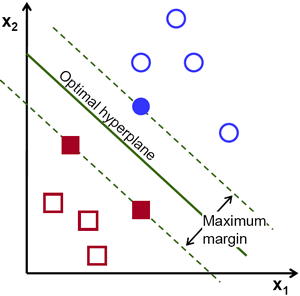
\includegraphics[width=0.5\textwidth]{optimal-hyperplane.png}
	\caption{Clustering: The process of regrouping showing high similarities into separate coherent groups}
\end{figure} 

\paragraph{Binary SVM}
Binary SVM is initially designed as a function classifying two sets of linearly
distinguishable  data. 
\paragraph{Multi-class SVM}
There  are  two  main  categories  of  multi-category  SVM.  One  is  constructed  by combining several binary classifiers, e.g., one-against-one SVM and one-against rest SVM. The other has only one classifier, in which all data are treated by one optimization formulation, as all-against-all method\cite{hsu2002comparison}.

\subparagraph{One againt-rest SVM}
One-against-rest method is probably the earliest approach implemented for multi-
class classification. Figure 3 shows a simple example of one-against-rest SVM applied to three class  recognition.   There  are  three  classifiers:  Class1  vs  Class(2,3);  Class2  vs Class(1,3) and Class3 vs Class(1,2).   Such kind of multi-class SVM is easy to understand and to compute.   However,  it exists large areas of difficult decision (overlapping of all areas), which are colored on Figure 2.1. In these case, the usual is to consider the classifier that has the largest margin as the "safer" decision.

\begin{figure}[h!]
	\centering
	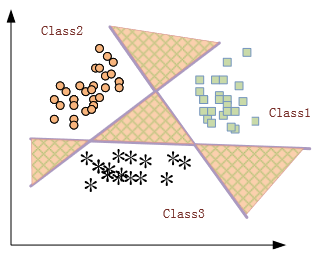
\includegraphics[width=0.5\textwidth]{one_against_rest.png}
	\caption{Diagram of one-against-rest SVM applied to a three-class classification problem}
\end{figure} 

\subparagraph{One-against-one SVM}
The one-against-one method is introduced in\cite{knerr1990single} , which constructs binary SVM classifiers for all pairs of classes, such as C1 against C2, C2 against C3, etc. For K class problem, the total number of binary SVMs is K(K−1)/2.

\begin{figure}[h!]
	\centering
	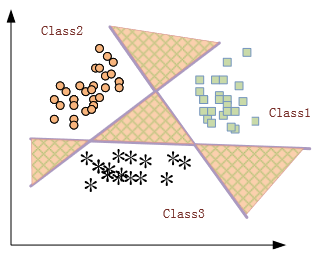
\includegraphics[width=0.5\textwidth]{one_against_rest.png}
	\caption{Diagram of one-against-rest SVM applied to a three-class classification problem}
\end{figure} 

\subparagraph{All-against-all SVM}
Similar to binary SVM, all-against-all method solves a
K class problem by addressing a single quadratic optimization problem of size
(K-1)/n. That is to say,it needs to find an optimal hyperplane for separating all classes\cite{hsu2002comparison}.

\begin{figure}[h!]
	\centering
	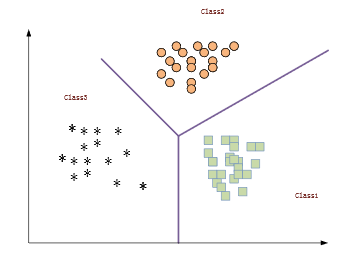
\includegraphics[width=0.5\textwidth]{all_against_all.png}
	\caption{Diagram of one-against-rest SVM applied to a three-class classification problem}
\end{figure} 

The mathematical development of the SVM all-against-all formulas is available and well described in\cite{bredensteiner1999multicategory}.

Three kinds of multi-class SVM approaches have been presented.  As far as the
training cost is concerned, one-against-rest SVM is preferable, because it needs
only K binary  SVMs.   However,  it  has  a  largest  areas  of  difficult  decision,  as shown by the comparison of Figures 2.1, 2.2 and 2.3.  Compared to one-against-all  SVM,  one-against-one  SVM  algorithm  is  more time-consuming. However, it generally performs better and is more suitable for practical use. Nevertheless, all these methods are usually applied in offline applications, in which test step can begin only when training step has
finished and all parameters of SVMs have been chosen\cite{lu2014online}.

\subsection{Application on Static Data}

Multiple examples can be given on how clustering can be applied in static data domains: 
\begin{itemize}
	\item One major clustering client is image processing. Having a finite number of images, multiple needs can exist weither it's histogramm clustering in order to recognise the most used colors or even to categorize the objects presented in the images.\cite{wu1993optimal}.
	\item The medical world presents itself as an essential candidate\cite{cios2002uniqueness}. Application vary from normal data extraction in order to improve patient's conditions to studying genome data in genetical engineering\cite{baldi2002dna}. 
	\item In the world of commerce clustering is used to regroup different types of customers in order to target them with marketing strategies built within their preferences.
\end{itemize}

Other aspects of daily life can also be included in this list of activities that benefit of clustering.

\section{Onine data streaming study}
Data stream mining is an active research area that has recently emerged to discover knowledge from large amounts of continuously generated data. For the last decade, we have seen an increasing interest in managing these massive, unbounded sequences of data objects that are continuously generated at rapid rates, the so-called data streams\cite{chandola2011knowledge}.

Applications of data streams include mining data generated by sensor networks,
meteorological analysis, stock market analysis, and computer network traffic monitoring, just to name a few. These applications involve data sets that are far too large to t in main memory and are typically stored in a secondary storage device. 

\subsection{Online incremental data mining needs}

For data stream mining, however, the successful development of algorithms
has to take into account the following restrictions:

\begin{itemize}
	\item Data objects arrive continuously.
	\item There is no control over the order in which the data objects should be processed.
	\item The size of a stream is (potentially) unbounded.
	\item Data objects are discarded after they have been processed. In practice, one can store part of the data for a given period of time, using a forgetting mechanism to discard them later.
	\item The unknown data generation process is possibly non-stationary, i.e., its probability distribution may change over time.
\end{itemize}

In conclusion of what is presented before, we can conclude that a need is presented in the form of data mining techniques that can at the same time perform in an incremental way and without going offline. These two factors have been the major study element of multiple techniques divided between supervised (data classification) and unsupervised (data clustering) technologies.

The rest of this paper will be presented as follows: Presentation of unsupervised learning techniques (data clustering) which function in an online incremental way, then the presentation of supervised learning techniques (data classification) which function in the same way followed by an analytical study of what's presented in this section.

\subsection{Data stream clustering techniques}

In this section multiple data clustering techniques will be presented and what these methodologies have in commun is the fact that the authors of these algorithms aimed to achieve what is close to optimal online incremental data clustering.

\subsubsection{DBSCAN}

One of the pioneer methodologies in data clustering technologies is DBSCAN. DBSCAN was presented the first time in 1996 \cite{ester1996density} where this algorithm presented the solution to multiple needs as dicovering clusters with arbitrary shape having small apriori knowledge of the arriving data.

This algorithm is essential in order to understand how will the data stream clustering algorithms function, since the majority of the newly discovered algorithms are related to DBSCAN in one way or another.



\subsubsection{Data Stream algorithms}
Data stream mining is an active research area that has recently emerged to discover knowledge from large amounts of continuously generated data. In this context, several data stream clustering algorithms have been proposed to perform unsupervised learning.

\paragraph{DenStream}

Multiple data stream clustering algorithms have been presented recently in order to achieve what is close to optimal online incremental data clustering. DenStream\cite{cao2006density} was first presented in 2009 in order to fulfill multiple needs in data mining:
\begin{itemize}
	\item No assumption on the number of clusters.  The number of clusters is often unknown in advance. Furthermore, in an evolving data stream, the num-
	ber of natural clusters is often changing.
	\item Discovery of clusters with arbitrary shape.  This	is very important for many data stream applications. For example, in network monitoring, the
	distribution of connections is usually irregular. In environmen observation, the layout of an area with similar environment conditions could be any shape.
	\item Ability to handle outliers.  In the data stream scenario, due to the influence of various factors, such as electromagnetic interference, temporary failure of sensors, weak battery of sensors, etc., some random noise appears occasionally.
\end{itemize}

Different approaches were presented trying to handle data streams\cite{hinneburg1998efficient}\cite{wang1997sting}\cite{aggarwal2004framework} but these methods were limited to knowing the amount of data that will be present as the entry of the system. Other methodologies didn't take into consideration the clusters of arbitrary shape either if they were one-pass methods\cite{charikar2003better}\cite{guha2003clustering}\cite{guha2003clustering} or even evolving methods\cite{aggarwal2003framework}...

DenStream consists of two major steps: The first is merging (cf. Algorithm 1)
\begin{figure}[h!]
	\centering
	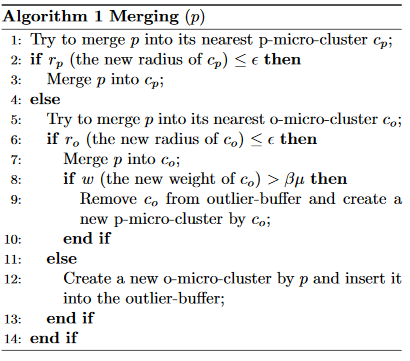
\includegraphics[width=0.5\textwidth]{merging.png}
	\caption{Clustering: The process of regrouping showing high similarities into separate coherent groups}
\end{figure} 

Zfter merging is done DenStream is applied over a certain period of time in order to have a check on the data periodically(cf. Algorithm 2).

\begin{figure}[h!]
	\centering
	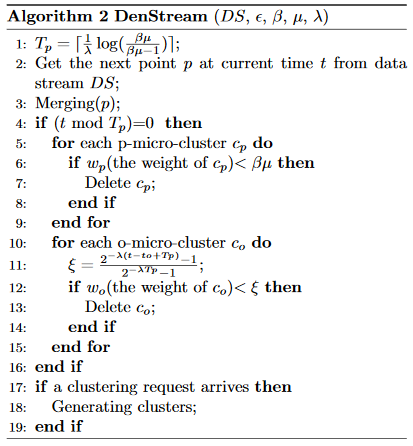
\includegraphics[width=0.5\textwidth]{DenStream.png}
	\caption{Clustering: The process of regrouping showing high similarities into separate coherent groups}
\end{figure} 

\paragraph{Clustream}

The CluStream method is a method of clustering data streams, based on the concept of microclusters. Microclusters are data structures which summarize a set of instances from the stream, and is composed of a set of statistics which are easily updated and allow fast analysis. 

CluStream has two phases. In the online phase, a set of microclusters are kept in main memory; each instance coming from the input stream can then be either appended to an existing microcluster or created as a new microcluster. Space for the new microcluster is created either by deleting a microcluster (by analyzing its expiration timestamp) or by merging the two closest microclusters. The offline phase will apply a weighted k-means algorithm on the microclusters, to obtain the final clusters from the stream\cite{ClustreamDefinition}.


\bibliographystyle{unsrt}
\bibliography{biblio}

\end{document}
